\title{Genetics and the History of Population Size}
\author{Alan R. Rogers}
\date{\today}
\frame{\titlepage}

\begin{frame}
\frametitle{Mismatch Distributions of Amerindian mtDNA Haplogroups}
\begin{columns}
\column{0.7\textwidth}
\includegraphics[height=0.8\textheight]{fagundesmm.png}
\column{0.3\textwidth}
\footnotesize Fagundes et al 2008
\end{columns}
\end{frame}

\begin{frame}
\frametitle{Genealogies of Amerindian mtDNA Haplogroups}
\centering
\includegraphics[width=0.9\textwidth]{fagundestree.png}%
\llap{\footnotesize Fagundes et al 2008}\\
\end{frame}

\begin{frame}
\frametitle{Estimated Size of Amerindian Population}
\includegraphics[width=0.9\textwidth]{fagundespop.png}%
\llap{\footnotesize Fagundes et al 2008}\\
\end{frame}

\begin{frame}
\frametitle{Estimated Size of Bison Population}
\includegraphics[width=0.9\textwidth]{bison.jpeg}
\end{frame}

\begin{frame}
\frametitle{What about the nuclear genome}

\begin{itemize}
\item Huge amounts of data.
\item Recombination makes previous methods unusable.
\end{itemize}
\end{frame}

\ifthenelse{\theshowthis=0}{
\begin{frame}
\frametitle{Deep History}
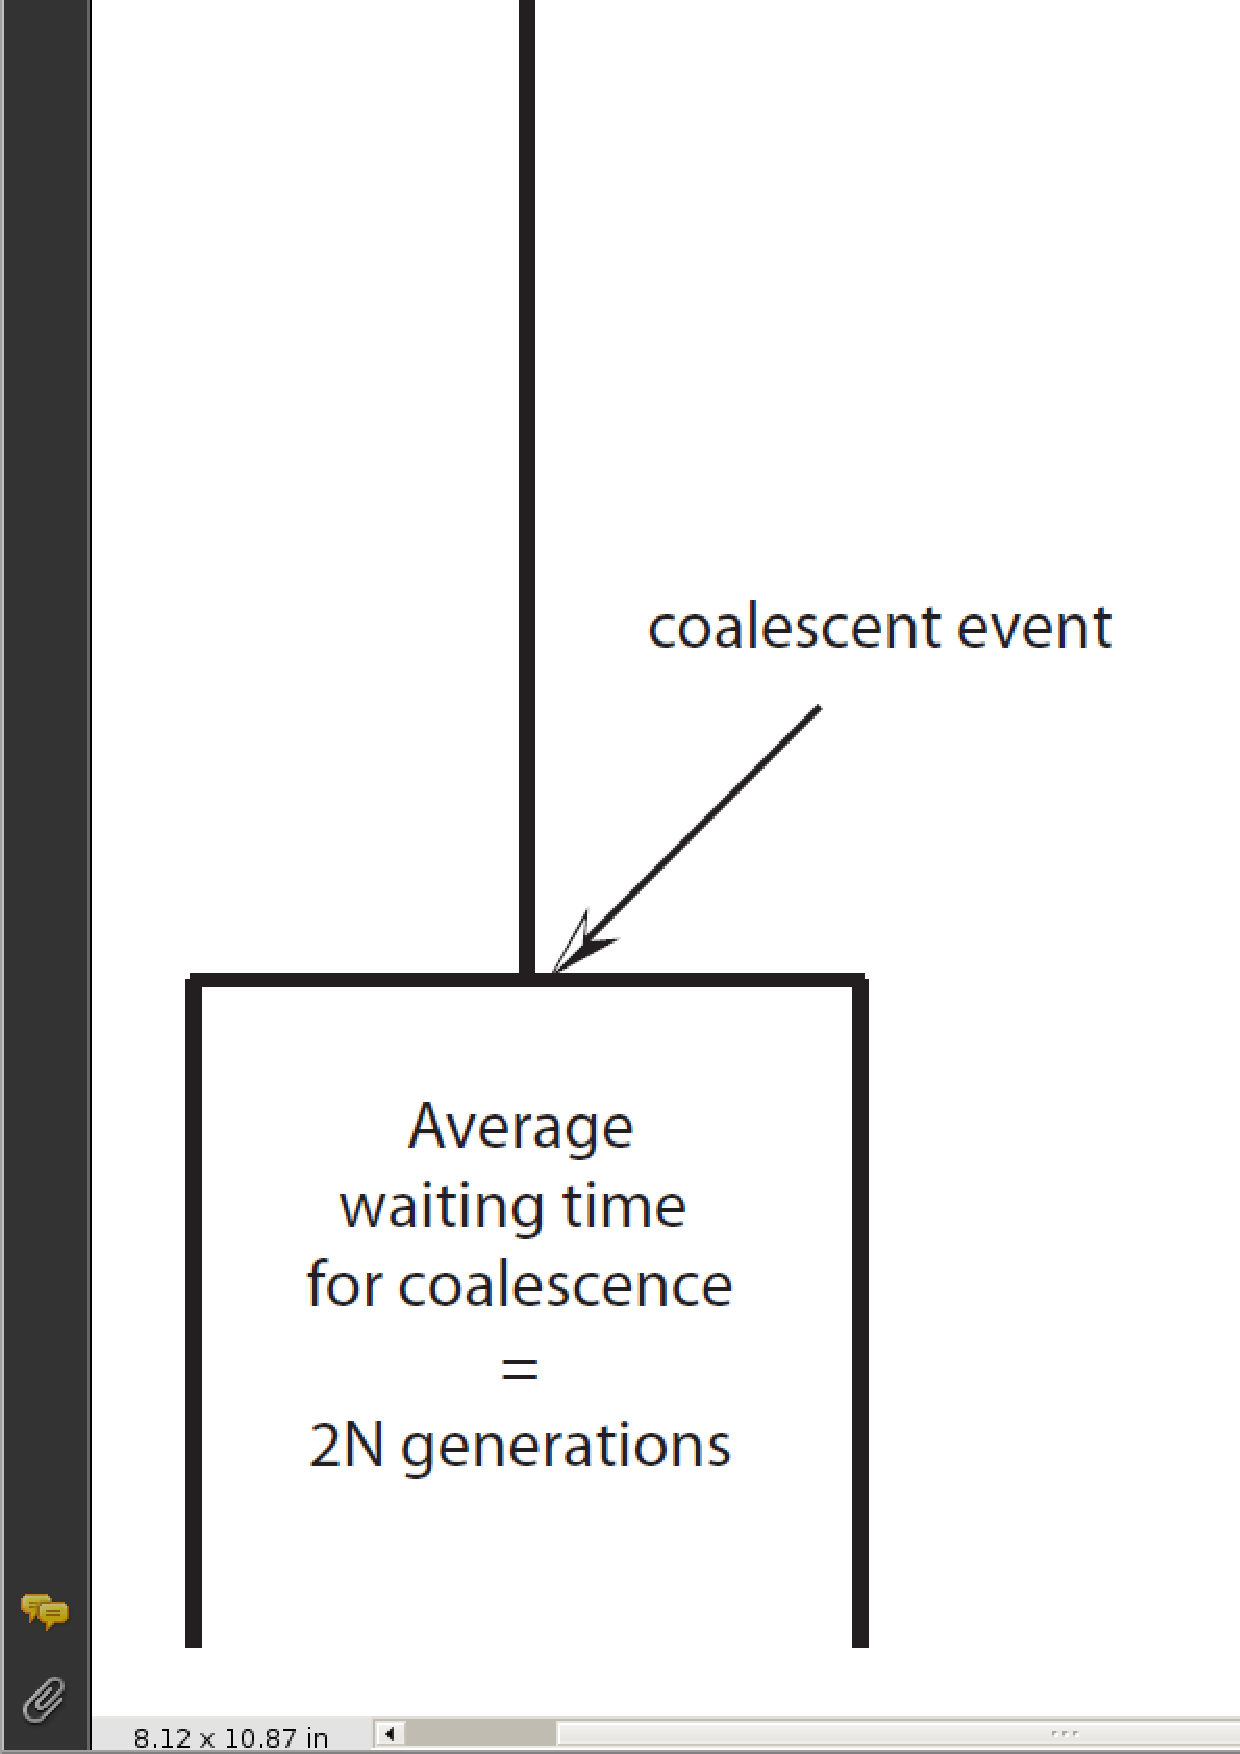
\includegraphics[height=0.8\textheight]{Huff-deeptree.png}
\footnotesize Huff et al 2010
\end{frame}

\begin{frame}
\frametitle{Deep History}
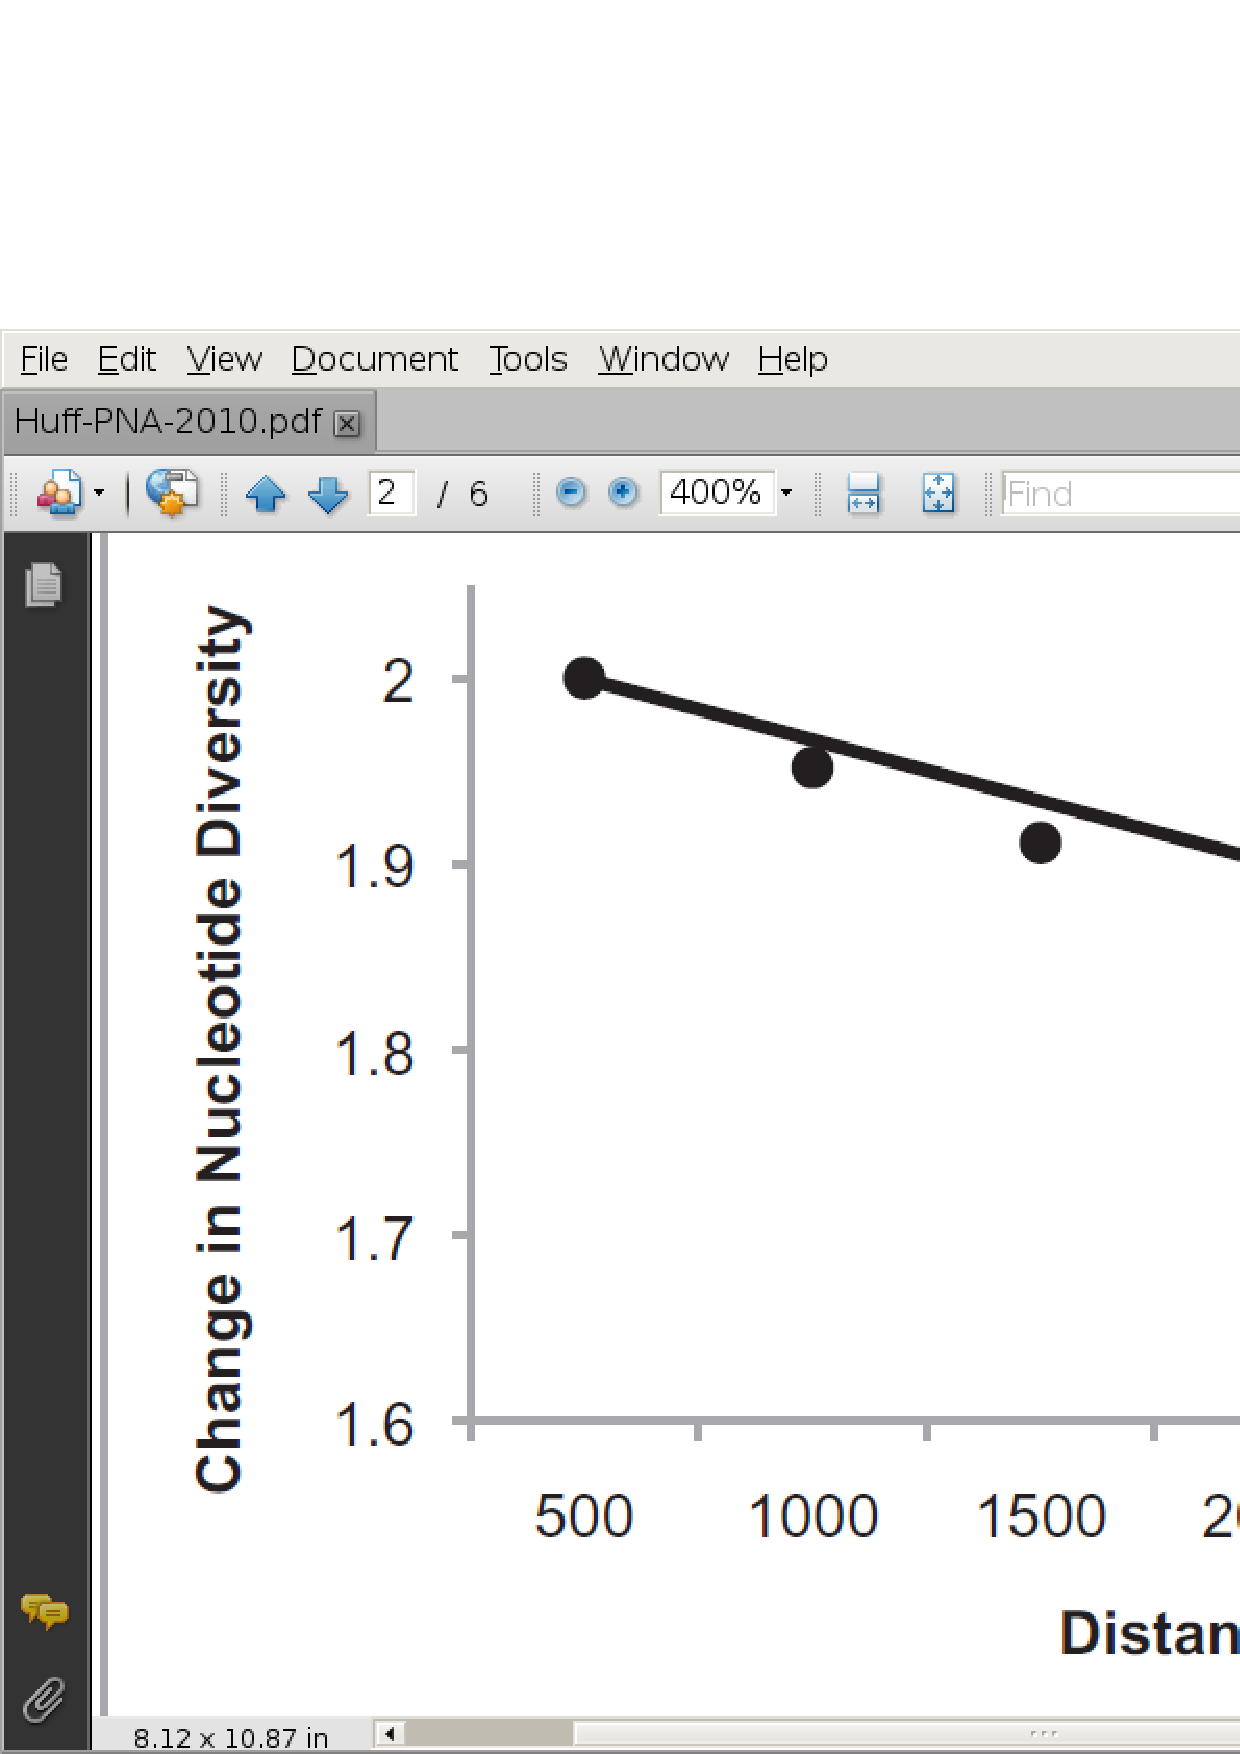
\includegraphics[width=\textwidth]{Huff-scatter.png}\\
\mbox{}\hfill\footnotesize Huff et al 2010
\end{frame}

\begin{frame}
\frametitle{Deep History}
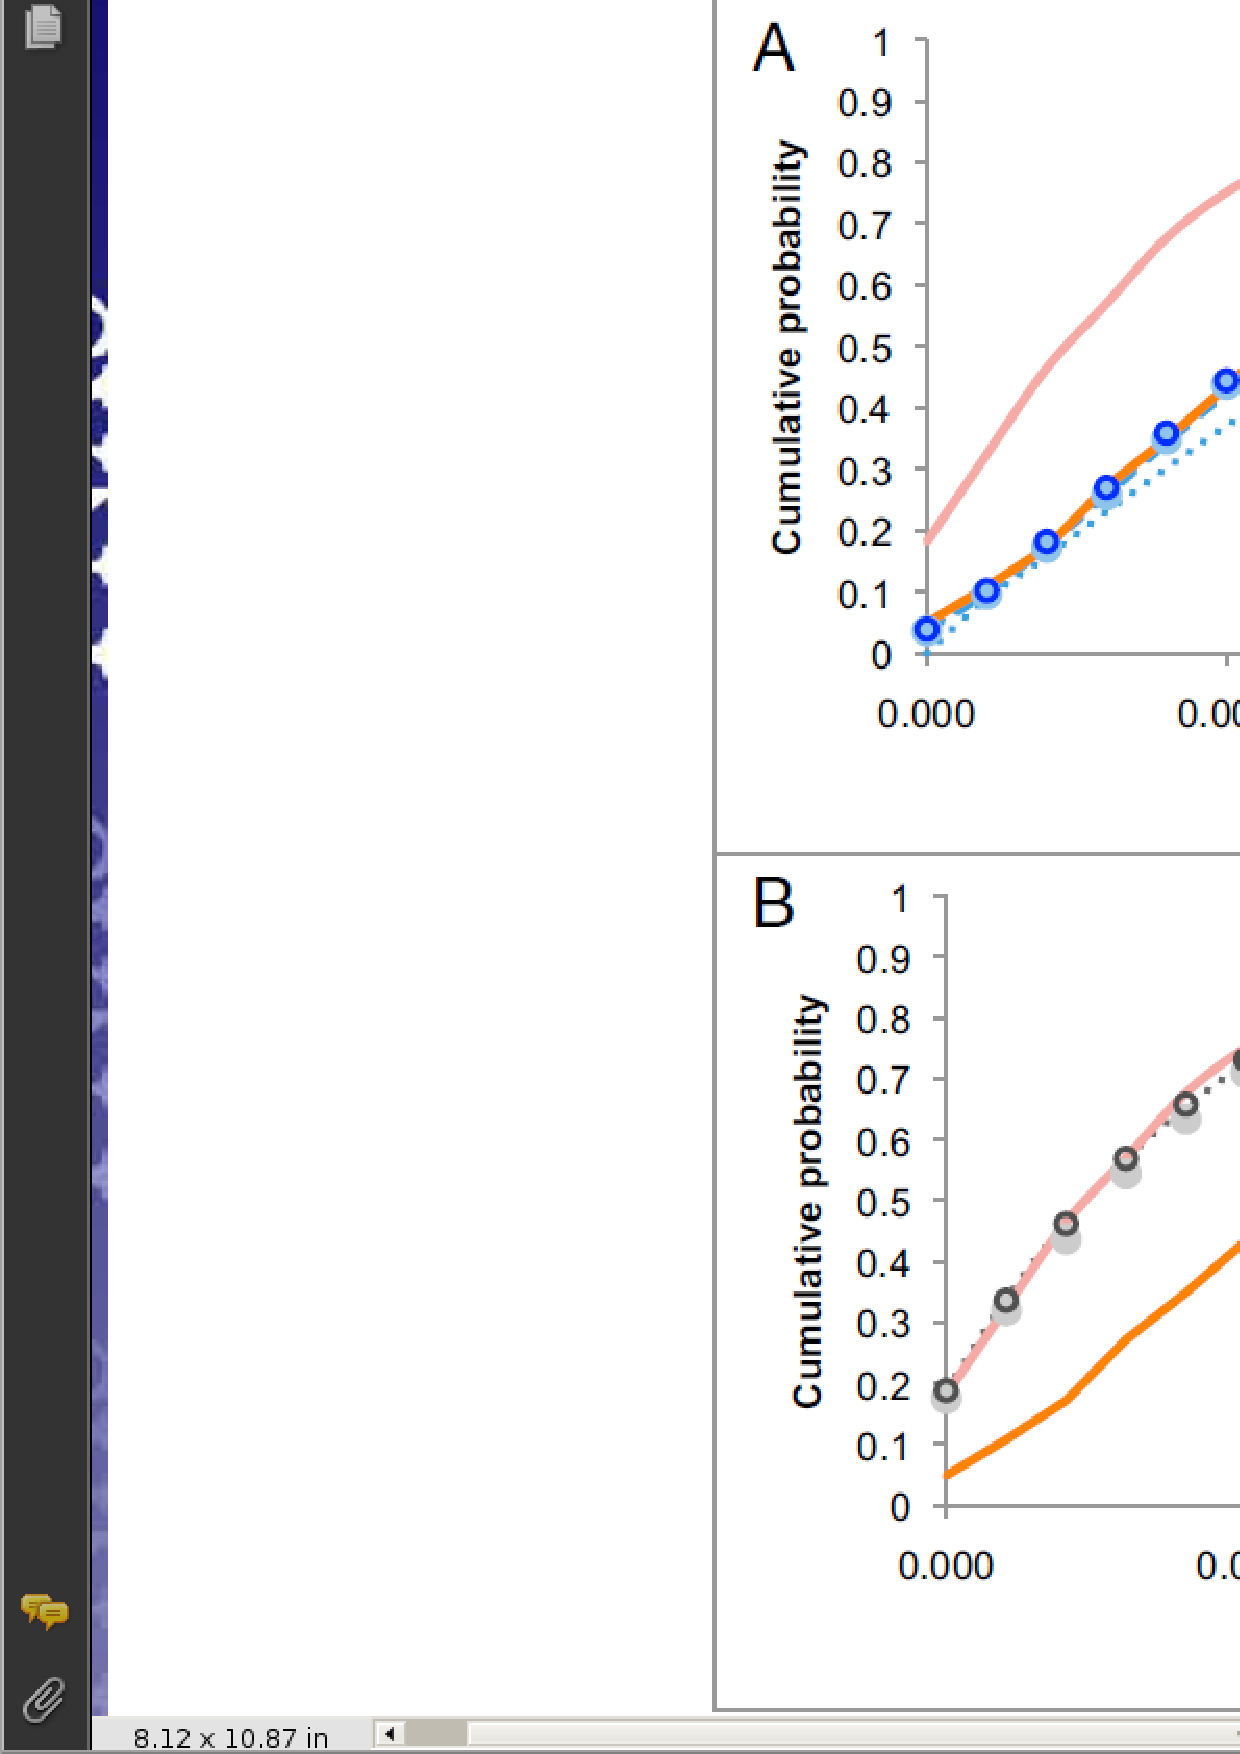
\includegraphics[height=0.8\textheight]{Huff-cumprob.png}\\
\mbox{}\hfill\footnotesize Huff et al 2010
\end{frame}

\begin{frame}
\frametitle{Deep History}
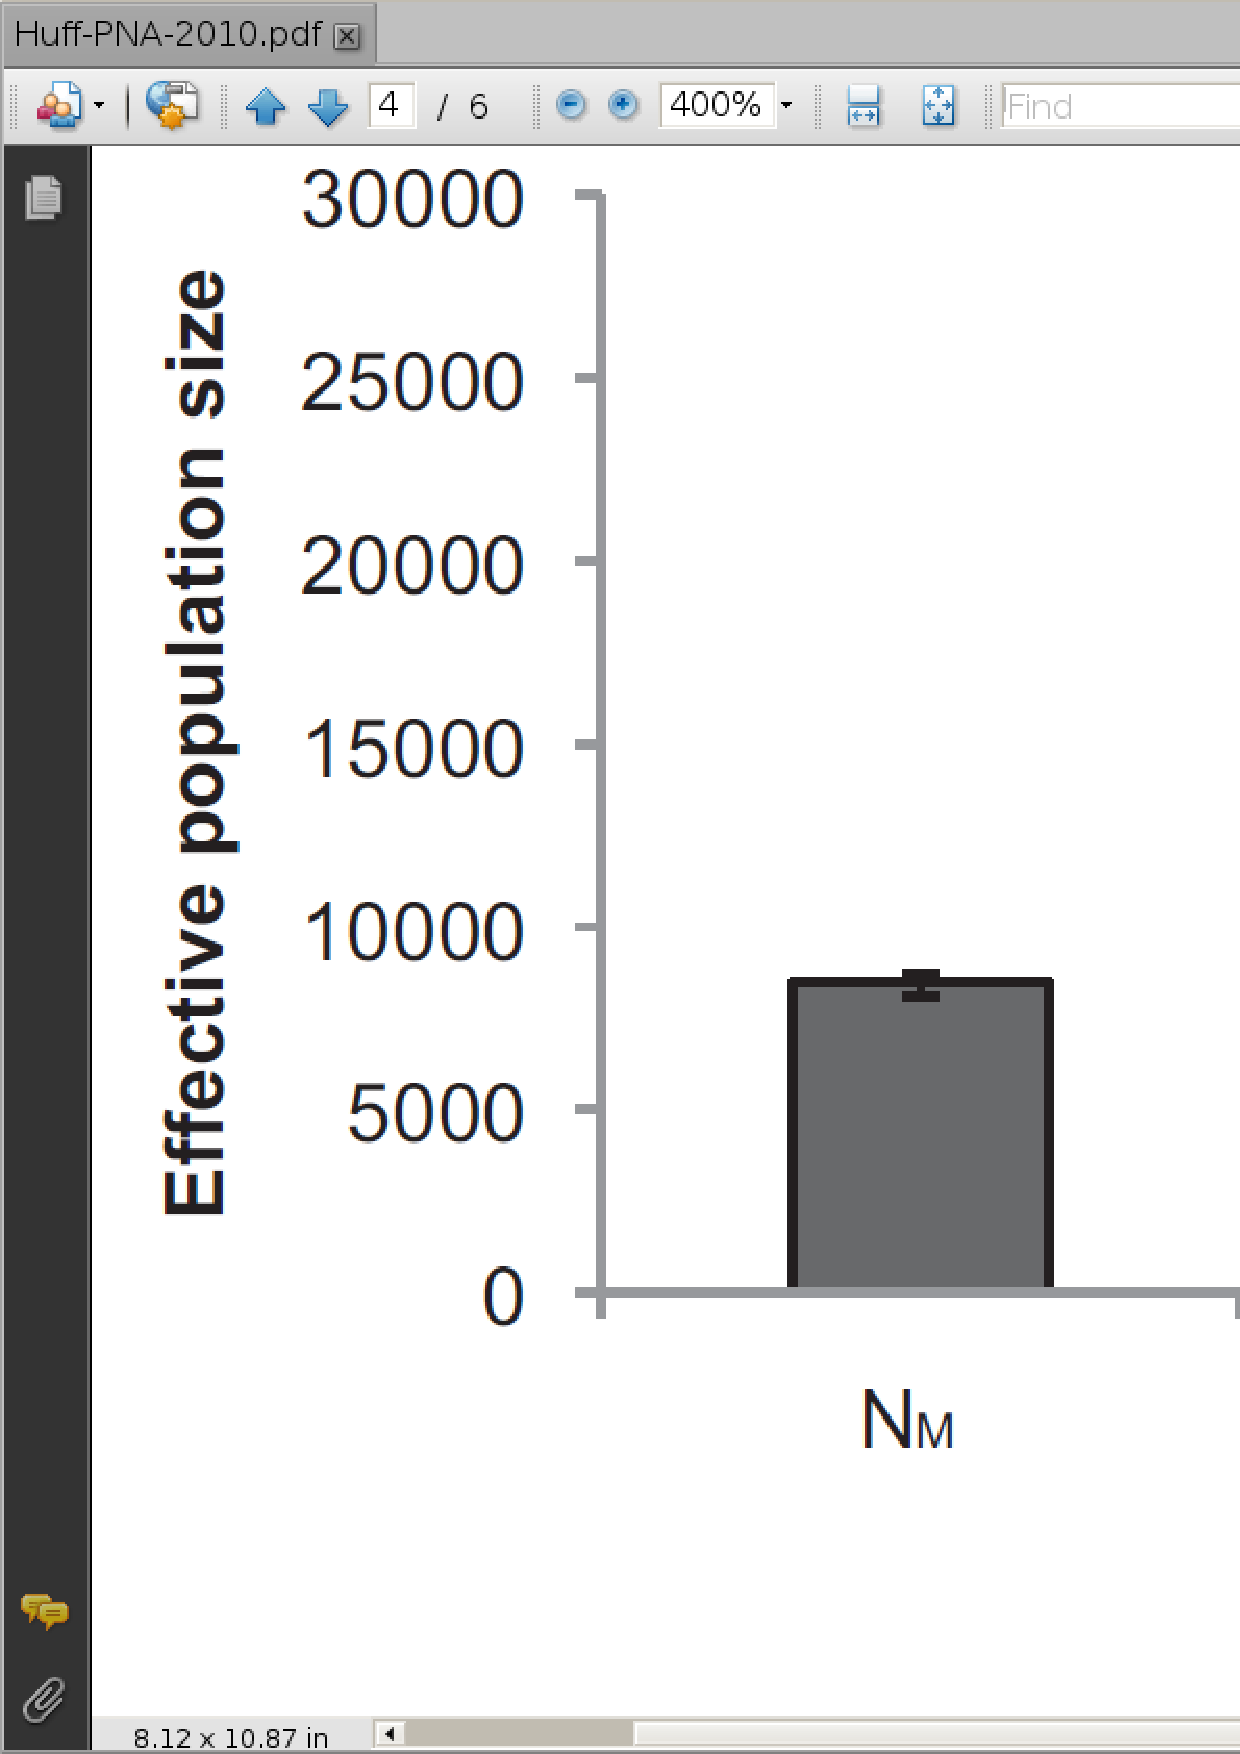
\includegraphics[width=\textwidth]{Huff-estimates.png}\\
\mbox{}\hfill\footnotesize Huff et al 2010
\end{frame}
}{}

\begin{frame}
\frametitle{PSMC: deep history from a single diploid genome}
\includegraphics[width=\textwidth]{prufer-pophist.jpg}\\[-2ex]
{\mbox{}\hfill\footnotesize Pr{\"u}fer et al 2014}

Accurate back to 2~mya. Not for last 20,000 years.
\end{frame}%

\begin{frame}
\begin{columns}
\column{0.7\textwidth}
\includegraphics[width=\linewidth]{stairway.png}
\column{0.35\textwidth}
\raggedleft
\textcolor{blue}{\large Stairway plot}

\bigskip

Uses site frequency spectrum.

\bigskip

Accomodates large samples. Can study last 20,000 years.

\bigskip

Liu \& Fu 2015
\end{columns}
\end{frame}

\begin{frame}
\frametitle{SMC++}
\includegraphics[width=\textwidth]{Terhorst-smcpp.png}\\

\small 8 modern populations and Ust'-Ishim (45-kya modern Siberian). Log
scale on left, arithmetic on right.  Combines advantages of PSMC and
spectrum. Large samples or small; accurate across both recent and deep
scales of time. (Terhorst et al. 2017)
\end{frame}
